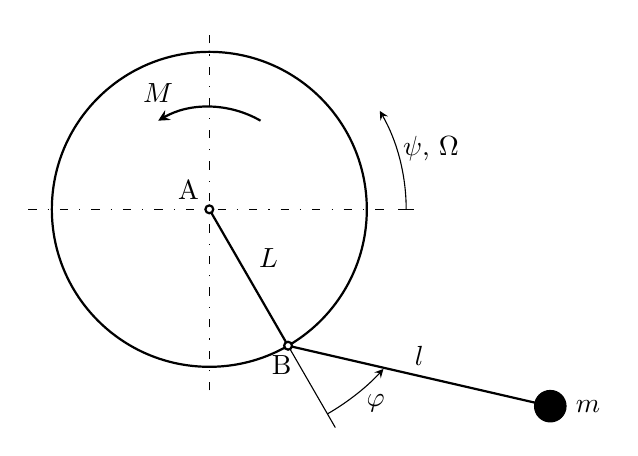
\begin{tikzpicture}[>=stealth]
\draw [loosely dashdotted] (-2.3,0) -- (2.3,0);
\draw [loosely dashdotted](0,-2.3) -- (0,2.3);
\draw [thick] (0,0) circle (2cm);


\draw [thick] (0mm,0mm) -- node[anchor=south west]{$L$} (-60:2);
%\draw (0,0) -- (-60:3);
%\draw [->] (-60:2.8cm) arc (-45:2.8cm:2.8cm);

\draw [->, thick] (60:1.3cm) arc (60:120:1.3cm) node[above=0.1cm]{$M$};

% Bemaßung Omega
\draw [->] (0:2.5cm) arc (0:30:2.5cm) node[right=0.65cm,below=0.2cm]{$\psi$, $\Omega$};
\draw  (2.4,0) -- (2.6,0);

% Bemaßung l und m
\draw  [thick] (-60:2) -- node[anchor=south]{$l$} (-30:5);
\filldraw (-30:5) circle (.2cm) node[right=0.2cm]{$m$};

% Bemaßung Winkel
\draw (-60:2) --  (-60:3.2);
\draw [->] (-60:3cm) arc (-60:-42.5:3cm) node[left=0.1cm, below=0.2cm]{$\varphi$};


% Einfügen der Punkte A und B
\filldraw[fill=white, draw=black, thick] (0,0) circle (0.05cm) node[anchor=south east]{A};
\filldraw[fill=white, draw=black, thick] (-60:2) circle (0.05cm) node[left=0.08cm,below]{B};
\end{tikzpicture}
